% TODO:
%  - Search for "FIX" and fix

\documentclass[12pt, twocolumn]{article}

\usepackage{mathtools}

\newcommand*{\eu}{e}
\newcommand*{\iu}{i}

\DeclarePairedDelimiter{\bra}{\langle}{\rvert}
\DeclarePairedDelimiter{\ket}{\lvert}{\rangle}
\DeclarePairedDelimiterX{\braket}[2]{\langle}{\rangle}
  {#1\,\delimsize\vert\,\mathopen{}#2}

\usepackage{biblatex}
\addbibresource{references.bib}

\usepackage[hidelinks]{hyperref}

\title{The Quantum Ising Chain as an Open Quantum System}
\author{David Basoco \and Jack Hetherington \and Davis Rash \and Tim Ross}
\date{December 6, 2023}

\begin{document}
  \maketitle

  \section{Introduction}
  The transverse-field Ising model is a quantum mechanical model of a spin lattice and can be simulated on a quantum computer. In one dimension the Hamiltonian describing the model, with periodic boundary conditions, is
  \begin{equation}
    \label{eq:system-hamiltonian}
    H = \sum_{i = 1}^{n} \sigma_{i}^{x} \sigma_{i + 1}^{x}
        + \sigma_{1}^{y} \sigma_{2}^{z} \dotsm \sigma_{n - 1}^{z} \sigma_{n}^{y}
        + \lambda \sum_{i = 1}^{n} \sigma_{i}^{z},
  \end{equation}
  where \( n = 8 \) in our case.

  The magnetization of the full Ising model can be evolved over time to analyze the effects of changes to parameters. To simulate the chain as an open quantum system, the Ising model is coupled to a decoherence channel at a single site. The system is represented in Fig.~\ref{fig:ising-chain-with-environment}.
  \begin{figure}%[!htb]
    \centering
    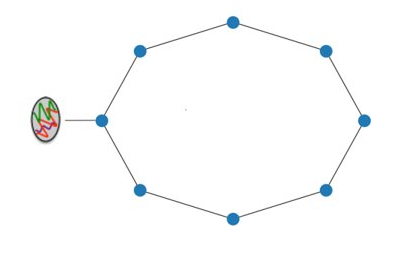
\includegraphics[width=\columnwidth]{images/ising_chain_with_environment.png}
    \caption{Representation of the system being studied.%
      \label{fig:ising-chain-with-environment}}
  \end{figure}
  Due to limitations of using the IBM quantum systems, and the large number of runs needed to get necessary data, the IBM QASM simulator was used for this project.

  \subsection{Applications}
  No quantum system is perfectly protected from the environment. Simulating the Ising model, with a known result, can provide information on what kinds of noise are present in an untested quantum computer. Including details on what type(s) of noise are affecting the system, and how strongly they impact it.

  \section{Quantum Gate Operations}
  The closed Ising model described by the Hamiltonian~\eqref{eq:system-hamiltonian} is diagonalized exactly by applying a unitary disentangling operator \( U_{\textnormal{dis}} \) such that
  \begin{equation}
    \tilde{H}
      = U_{\textnormal{dis}}^{\dagger} H
        U_{\textnormal{dis}}^{\vphantom{\dagger}},
  \end{equation}
  where \( \tilde{H} \) is a noninteracting Hamiltonian. For the Ising model, the method to obtain the \( U_{\textnormal{dis}} \) is threefold.
  \begin{enumerate}
    \item We first need to map spins to fermionic modes with the Jordan--Wigner transform. If this step is required varies depending on the hardware involved, in our case it was not required. % FIX this is not true
    \item The fermionic modes are mapped to momentum space by applying a Fourier transform.
    \item A Bogoliubov transform decouples the modes in opposite momenta.
  \end{enumerate}
  The successive application of these three transformations is our unitary disentangling operator
  \begin{equation}
    % FIX confirm the order of these. Are they JW-FT-Bog for the inverse (dagger) case, or this one?
    U_{\textnormal{dis}}
      = U_{\textnormal{JW}} U_{\textnormal{FT}} U_{\textnormal{Bog}}.
  \end{equation}

  \subsection{Fast Fermionic Fourier Transform}
  Now we need to get the fermionic modes to momentum space with the quantum Fourier Transform
  \begin{equation}
    \label{eq:qft}
    b_{k}
      = \frac{1}{\sqrt{n}}
        \sum_{j = 1}^{n} \eu^{2 \pi \iu j k / n} c_{j}, \qquad
    k = -\frac{n}{2} + 1, \dotsc, \frac{n}{2}
  \end{equation}
  Although this is valid in general, we have \( n = 2^{m} \), permitting us to use the fast Fourier transform. The resulting Hamiltonian is
  \begin{equation}
    H_{b}
      = \sum_{k = -n / 2 + 1}^{n / 2}
        \biggl[
          2 \biggl( \lambda - \cos \frac{2 \pi k}{n} \biggr)
          b_{k}^{\dagger} b_{k}^{\vphantom{\dagger}}
          + \iu \sin \biggl( \frac{2 \pi k}{n} \biggr)
            (b_{-k}^{\dagger} b_{k}^{\dagger}
             - b_{-k}^{\vphantom{\dagger}} b_{k}^{\vphantom{\dagger}})
        \biggr].
  \end{equation}

  \subsection{Bogoliubov Transform}
  The final step is to decouple the modes that have opposite momenta using the Bogoliubov transformation
  \begin{subequations}
    \begin{align}
      a_{k}
        &= u_{k}^{\vphantom{\dagger}} b_{k}^{\vphantom{\dagger}}
           + \iu v_{k}^{\vphantom{\dagger}} b_{-k}^{\dagger}, \\
      a_{k}^{\dagger}
        &= u_{k}^{\vphantom{\dagger}} b_{k}^{\dagger}
           + \iu v_{k}^{\vphantom{\dagger}} b_{-k}^{\vphantom{\dagger}},
    \end{align}
  \end{subequations}
  which corresponds to a matrix equation with the solution
  \begin{equation}
    B_{k}^{n}
      = \begin{pmatrix}
              \cos(\theta_{k} / 2) & 0 & 0 & \iu \sin(\theta_{k} / 2) \\
                                 0 & 1 & 0 &                        0 \\
                                 0 & 0 & 1 &                        0 \\
          \iu \sin(\theta_{k} / 2) & 0 & 0 &     \cos(\theta_{k} / 2)
      \end{pmatrix}
  \end{equation}
  where
  \begin{equation}
    \theta_{k}
      = \arccos
        \frac{\lambda - \cos(2 \pi k / n)}
             {\sqrt{(\lambda - \cos(2 \pi k / n))^{2} + \sin^{2}(2 \pi k / n)}}.
  \end{equation}
  As a result
  \begin{equation}
    \tilde{H}
      = H_{a}
      = \sum_{k = -n / 2 + 1}^{n / 2}
        \omega_{k}^{\vphantom{\dagger}} a_{k}^{\dagger}
        a_{k}^{\vphantom{\dagger}}
  \end{equation}
  where
  \begin{equation}
    \omega_{k}
      = \sqrt{\biggl( \lambda - \cos \frac{2\pi k}{n} \biggr)^{2}
              + \sin^{2} \frac{2\pi k}{n}}.
  \end{equation}

  \section{Time Evolution}
  With \( U_{\textnormal{dis}} \) applied to the basis states we exactly time evolve the problem. The time evolution for a given state using the time-independent Hamiltonian is described using the time evolution unitary \( U(t) = \eu^{-\iu t H} \):
  \begin{equation}
    \ket{\psi(t)}
      = U(t) \ket{\psi_{0}}
      = \sum_{i} \eu^{-\iu t \epsilon_{i}} \ket{E_{i}} \braket{E_{i}}{\psi_{0}},
  \end{equation}
  where \( \ket{\psi_{0}} \) is the initial state and \( \epsilon_{i} \) are the corresponding energies of the Hamiltonian states \( \ket{E_{i}} \). If an observable \( M \) is such that \( [H, M] \neq 0 \), then \( \langle M \rangle \) shows an oscillation in time
  \begin{equation}
    \langle M(t) \rangle
      = \sum_{i, j} \eu^{-\iu t (\epsilon_{i} - \epsilon_{j})}
        \braket{\psi_{0}}{E_{j}} \bra{E_{j}} M \ket{E_{i}}
        \braket{E_{i}}{\psi_{0}}.
  \end{equation}

  We now have computational basis states from the eigenstates \( \tilde{H} \) and all energies \( \epsilon_{i} \). We can construct the time evolution for a given state \( \ket{\psi_{0}} \) by expressing it in the computational basis and adding the corresponding factors \( \eu^{-\iu t \epsilon_{i}} \). The wave form expression can be presented analytically as
  \begin{equation}
    \langle \sigma_{z} \rangle
      = \frac{1 + 2 \lambda^{2} + \cos \bigl( 4 t \sqrt{1 + \lambda^{2}} \bigr)}
             {2 + 2 \lambda^{2}}.
  \end{equation}
  These steps are represented only briefly in the code but perform the function to obtain the expectation value of transverse magnetization \( M_{z} = \frac{1}{2} \langle \sigma_{z} \rangle \).

  \section{Open Quantum Decoherence Channels}
  Having created the closed system, we will now couple \( q_{0} \) to a surrounding environment. We will apply two decoherence channels across this coupling and observe the change in magnetization over time.

  \subsection{Amplitude Damping Channel}
  For an arbitrary pure state of the system \( \ket{\psi}_{s} = \alpha \ket{0}_{s} + \beta \ket{1}_{s} \), and setting the state of the environment to vacuum \( \ket{0}_{e} \), the two gates between the system and environment qubits transform the joint state into
  \begin{equation}
    \alpha \ket{0}_{1} \ket{0}_{2} + \beta \cos \theta \ket{1}_{1} \ket{0}_{2}
    + \beta \sin \theta \ket{0}_{1} \ket{1}_{2}.
  \end{equation}
  where \( q_{1} \) and \( q_{2} \) are the system and environment qubits, respectively. Therefore, identifying the states \( \ket{0}_{1} \) and \( \ket{1}_{1} \) with the ground state and excited states, respectively, and by choosing \( \theta = \arccos c_{1}(t) \), we get a reduced state of the system such that
  \begin{equation}
    \rho_{s}(t)
      = \begin{pmatrix}
          \lvert c_{1}(t) \rvert^{2} & c_{0}^{*} c_{1}(t)             \\
          c_{0} c_{1}^{*}(t)         & 1 - \lvert c_{1}(t) \rvert^{2}
        \end{pmatrix}
  \end{equation}
  These factors \( c_{0} \) and \( c_{1} \) are time-dependent factors of the wave equation. With a decay rate \( \gamma(t) \) from
  \begin{equation}
    \gamma(t) = -2 \mathcal{R} \biggl[ \frac{\dot{c}_{1}(t)}{c_{1}(t)} \biggr],
  \end{equation}
  with
  \begin{equation}
    c_{1}(t)
      = c_{1}(0) \eu^{-\lambda t / 2}
        \biggl[
          \cosh \biggl( \frac{\lambda t}{2} \sqrt{1 - 2 R} \biggr)
          + \frac{1}{\sqrt{1 - 2 R}}
            \sinh \biggl( \frac{\lambda t}{2} \sqrt{1 - 2 R} \biggr)
        \biggr].
  \end{equation}
  The application of this channel resulted in a lower average magnetization of the system. Notably it did not affect amplitude or frequency in time of the magnetization envelope. Nor did it show a decay affect on the magnetization.

  FIGURE HERE

  \subsection{Depolarizing Channel}
  The depolarization channel applied over time will move the system into an \( \frac{I}{2} \) state. The rate of this decoherence is affected by a decay-rate parameter \( \gamma \), which was kept constant at 0.5 for all runs. As shown by the following graph, the magnetization of the system decreases over time while coupled to the system. Since the depolarizing channel is only coupled at a single site, the decrease in energy applied to the single site must be propagating through the system and decreasing the magnetization of the whole system, but the affect of the transverse field prevents the system from going all the way into the \( \frac{I}{2} \) state. The three values of \( \lambda \) were graphed with the depolarizing channel, as shown in the figures. The effect of the depolarization channel is most noticeable with the higher value of \( \lambda \), see Fig.~\ref{fig:DepolChannelLambda18},  but the decrease in magnetization can also be seen in the lower \( \lambda \)'s in Fig.~\ref{fig:DepolChannelLambda05} and Fig.~\ref{fig:DepolChannelLambda09} .

  \begin{figure}%[!htb]
    \centering
    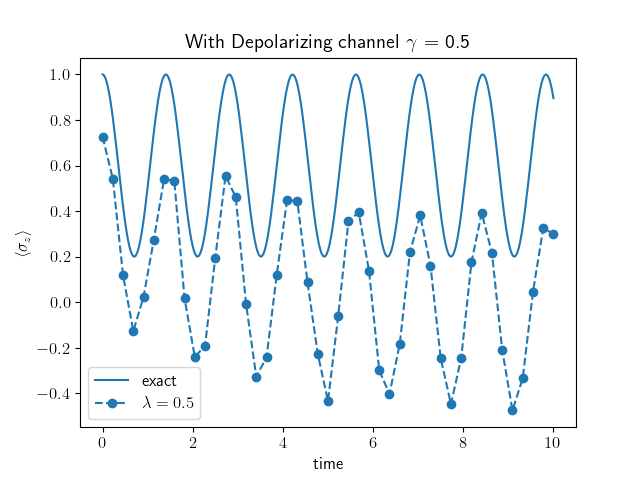
\includegraphics[width=\columnwidth]{images/DepolChannelLambda05.png}
    \caption{Time evolution of the Ising model coupled to a depolarizing channel with \( \lambda = 1.8 \).%
      \label{fig:DepolChannelLambda05}}
  \end{figure}

  \begin{figure}%[!htb]
    \centering
    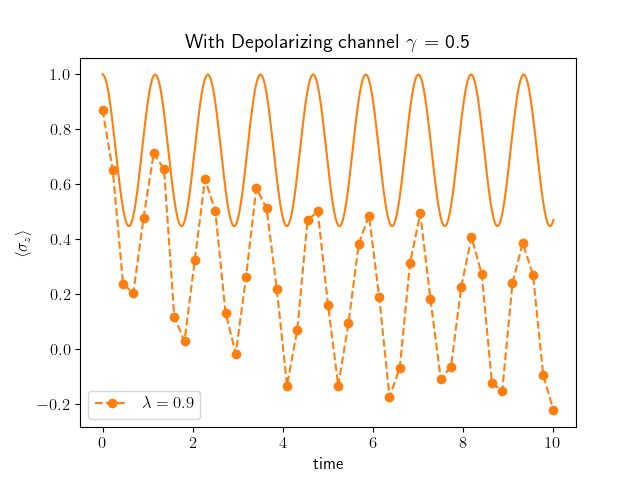
\includegraphics[width=\columnwidth]{images/DepolChannelLambda09.png}
    \caption{Time evolution of the Ising model coupled to a depolarizing channel with \( \lambda = 1.8 \).%
      \label{fig:DepolChannelLambda09}}
  \end{figure}

  \begin{figure}%[!htb]
    \centering
    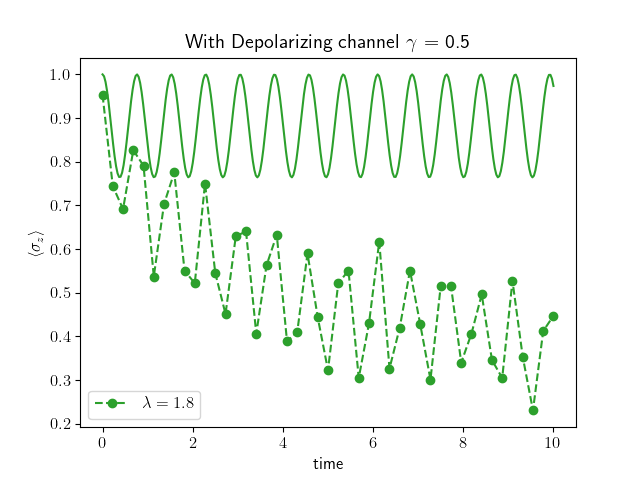
\includegraphics[width=\columnwidth]{images/DepolChannelLambda18.png}
    \caption{Time evolution of the Ising model coupled to a depolarizing channel with \( \lambda = 1.8 \).%
      \label{fig:DepolChannelLambda18}}
  \end{figure}

  \section{Results}

  Each type of noise affects the Ising model simulation differently, some examples include the amplitude damping channel causes a shift down in the total magnetization and the depolarizing channel causes the magnetization to decay over time. These distinct differences allow us to determine what types of noise are present in a system, and how strong each type is as well. This will be helpful in determining what types of noise and how much noise will need to be worked around in a given quantum computer.

  \printbibliography
\end{document}
